\chapter{Lecture 24/03/2025}

$$
\dot z = - \gamma z + \omega \xi(t) \leftrightarrow dz = - \gamma z dt + \omega dW
$$

$$
\dfrac{\partial \rho} {\partial t} = \dfrac{\partial}{\partial z} (\gamma z \rho) + \dfrac{\omega^2}{2} \dfrac{\partial^2 \rho}{\partial z^2}
$$

\dots

Consider a system with a quadratic potential given by
$$
U(z) = \frac{\gamma}{2}\,z^2.
$$
In the absence of noise, the deterministic dynamics drive the system toward the minimum of the potential, so that
$$
z(t) \to 0.
$$

When we add a stochastic perturbation, the dynamics can be modeled by the Langevin equation
$$
\dot{z} = -\gamma\,z + \omega\,\xi(t),
$$
where $\omega$ quantifies the noise strength and $\xi(t)$ is a white noise process. (Note that the negative sign in front of $\gamma$ ensures stability around $z=0$.) In the stationary regime, the fluctuations of $z$ are characterized by the variance
$$
\sigma^2 = \frac{\omega^2}{2\gamma}.
$$

Assuming that the system reaches a steady state, its stationary probability density function (PDF) is given by the Boltzmann distribution,
$$
P_s(z) = \frac{1}{\sqrt{2\pi\,\sigma^2}}\exp\left(-\frac{z^2}{2\sigma^2}\right).
$$
Substituting $\sigma^2 = \frac{\omega^2}{2\gamma}$, we obtain
$$
P_s(z) = \frac{1}{\sqrt{2\pi\,\frac{\omega^2}{2\gamma}}}\exp\left(-\frac{z^2}{\omega^2/\gamma}\right)
= \sqrt{\frac{\gamma}{\pi\,\omega^2}}\exp\left(-\frac{\gamma\,z^2}{\omega^2}\right).
$$

This stationary PDF describes how the probability of finding the system at a value $z$ is distributed. In particular:

\begin{itemize}
    \item \textbf{For weak noise} ($|\omega| \ll 1$): The variance $\sigma^2 = \omega^2/(2\gamma)$ is very small, so the distribution $P_s(z)$ becomes sharply peaked around $z=0$. In the limit of vanishing noise, $P_s(z)$ approaches a Dirac delta function, indicating that the system is almost surely at the equilibrium $z=0$.
    
    \item \textbf{For strong noise} ($|\omega| \gg 1$): The variance is large, which results in a broad stationary PDF. The probability spreads over a wider range of $z$ values, reflecting significant fluctuations around the equilibrium.
\end{itemize}

In summary, the behavior of the stationary PDF,
$$
P_s(z) = \sqrt{\frac{\gamma}{\pi\,\omega^2}}\exp\left(-\frac{\gamma\,z^2}{\omega^2}\right),
$$
is controlled by the noise intensity $\omega$ and the potential curvature $\gamma$. For small $\omega$, the distribution is narrowly concentrated (nearly a Dirac delta), while for large $\omega$, it becomes broad, indicating more pronounced stochastic fluctuations.


\newpage

\section{Stochastic Relaxation to Equilibrium}

Suppose we wish to study the differential equation
$$
\dot{y} = \gamma (b - y) + \omega\,\xi(t),
$$
which describes a system relaxing toward an equilibrium value $b$ with rate $\gamma$, perturbed by a stochastic force $\omega\,\xi(t)$ (with $\xi(t)$ being a white noise process).

To analyze the fluctuations around the equilibrium, we introduce the variable
$$
z = y - b \quad \Longrightarrow \quad y = b + z.
$$
Substituting this into the original equation yields
$$
\dot{z} = -\gamma\,z + \omega\,\xi(t).
$$

In the deterministic case (i.e., when $\omega=0$), the equation for the deterministic component $y_d$ is
$$
\dot{y}_d = \gamma (b - y_d).
$$
This equation has the solution
$$
y_d(t) \to b \quad \text{as} \quad t \to \infty,
$$
indicating that, in the absence of noise, the system relaxes exponentially to the equilibrium $b$.

When the stochastic term is present, the fluctuations $z$ about $b$ are governed by
$$
\dot{z} = -\gamma\,z + \omega\,\xi(t).
$$
At long times, the system reaches a stationary state in which $z$ is a Gaussian random variable with zero mean and variance
$$
\sigma^2 = \frac{\omega^2}{2\gamma}.
$$

Thus, for large $t$ the full solution behaves as
$$
y(t) \sim b + \mathcal{N}\Bigl(0, \frac{\omega^2}{2\gamma}\Bigr),
$$
or equivalently, in terms of the deviation $z$,
$$
z_{\text{cl}}(t) \sim \mathcal{N}\Bigl(0, \frac{\omega^2}{2\gamma}\Bigr) \quad \text{as} \quad t \to \infty.
$$

This analysis shows that while the deterministic part drives the system to the equilibrium $b$, the stochastic fluctuations cause the state to be distributed around $b$ according to a normal distribution with variance $\omega^2/(2\gamma)$.


\newpage

% Suppose $x_e$ to be an equilibrium point of the system $F(x)$:

% $$
% \begin{cases}
% \dot x = F(x) + \omega \xi(t) \\
% F(x_e) = 0
% \end{cases}
% $$

% $$
% F(y) = F[x_e + (y - x_e)] = F[x_e] + F'[x_e](y - x_e) + O(y - x_e)^2
% $$

% The case where the equilibrium is unstable is not interersting, so we will consider the case where the equilibrium is stable:

% $$
% \dot y \simeq F'(y_e)(y - y_e) + \omega \xi(t)
% $$

% $$
% F'(y_e) < 0
% \qquad \rightarrow \qquad
% F'(y_e) = - \gamma, \quad - \gamma> 0 
% $$

% $$
% \dot y = - \gamma (y - y_e) + \omega \xi(t) = \gamma (y_e - y) + \omega \xi(t)
% $$

% ---

% $$
% \dot z = -\gamma z + \omega \xi(t), z(0) = 0
% $$
% $$
% z -> gaussian <-> W_0N_0
% $$
% $$
% <z> = 0
% $$
% $$
% |\sigma^2(t)| = M \qquad \sigma^2(t) \to \dfrac{\omega^2}{2\gamma} \cancel{\leftrightarrow} WN \quad Var(\dots) = \infty
% $$
% $$
% <z(t)z(t+h)> \to \dfrac{\omega^2}{2\gamma} e ^{-\gamma |h|}
% $$
% this one behaves as a dirak delta function

% $$
% \boxed{\omega = c \gamma}
% $$
% $$
% \dot z = -\gamma z + c \gamma \xi(t) 
% $$
% $$
% \dot z = - \dfrac 1\delta z + \dfrac 1\delta \xi(t)
% $$
% $$
% \begin{cases}
%     R_z = \dfrac{c^2}{2} \gamma e ^{- \gamma |h|} \\
%     R_z(0) = \dfrac{c^2}{2} \gamma
% \end{cases}
% $$

% $$
% \int_{-\infty}^{+\infty} R_z(h) dh = \int_{-\infty}^{+\infty} \dfrac{c^2}{2} \gamma e ^{- \gamma |h|} dh = \dfrac{c^2}{\cancel 2} \cancel 2 \int_{0}^{+\infty} \gamma e ^{- \gamma h} dh = c^2
% $$

% for small characteristical  $\tau$ so this is a very good approximation for a white noise

% $$
% \lim_{\gamma \to + \infty} R_z(h; \gamma) = \delta(h)
% $$

\newpage
\section{Linearization around a Stable Equilibrium and Noise Scaling}

Suppose $x_e$ is an equilibrium point of the deterministic system
$$
\dot{x} = F(x),
$$
so that
$$
F(x_e)=0.
$$
In the presence of stochastic perturbations, the dynamics are described by
$$
\dot{x} = F(x) + \omega\,\xi(t),
$$
where $\omega\,\xi(t)$ represents an additive noise term with $\xi(t)$ as white noise.

To study the behavior near the equilibrium, we expand $F(x)$ about $x_e$. Let $y$ denote a variable so that
$$
F(y) = F\bigl[x_e + (y - x_e)\bigr] = F(x_e) + F'(x_e)(y - x_e) + O((y - x_e)^2).
$$
Since $F(x_e)=0$, for small deviations we have
$$
F(y) \approx F'(x_e)(y - x_e).
$$

For a stable equilibrium we require
$$
F'(x_e) < 0.
$$
We define
$$
F'(x_e) = -\gamma, \qquad \gamma>0.
$$
Thus, the linearized dynamics become
$$
\dot{y} \simeq -\gamma\,(y - x_e) + \omega\,\xi(t).
$$

It is convenient to introduce the deviation variable
$$
z = y - x_e \quad \Longrightarrow \quad y = x_e + z.
$$
Then the dynamics simplify to
$$
\dot{z} = -\gamma\,z + \omega\,\xi(t), \qquad z(0)=0.
$$

The solution $z(t)$ is a Gaussian process with mean
$$
\langle z(t)\rangle = 0,
$$
and in the stationary state, its variance is given by
$$
\sigma^2 = \frac{\omega^2}{2\gamma}.
$$
Moreover, the autocorrelation function is
$$
\langle z(t)\,z(t+h)\rangle = \frac{\omega^2}{2\gamma}\,e^{-\gamma|h|}.
$$
This autocorrelation decays exponentially with a characteristic time $1/\gamma$. In the limit of rapid relaxation ($\gamma \to \infty$), the autocorrelation function becomes sharply peaked and tends toward a Dirac delta function.

To formalize this limit, we introduce a scaling relation between the noise intensity and the relaxation rate by setting
$$
\boxed{\omega = c\,\gamma,}
$$
with $c$ a constant. Under this scaling, the SDE for $z$ becomes
$$
\dot{z} = -\gamma\,z + c\,\gamma\,\xi(t).
$$
Alternatively, by defining $\delta = \frac{1}{\gamma}$, the equation can be written as
$$
\dot{z} = -\frac{1}{\delta}\,z + \frac{c}{\delta}\,\xi(t).
$$

The autocorrelation function for $z$ then reads
$$
R_z(h) = \frac{c^2}{2}\,\gamma\,e^{-\gamma|h|}, \qquad R_z(0) = \frac{c^2}{2}\,\gamma.
$$
Its total area is given by
$$
\int_{-\infty}^{+\infty} R_z(h)\,dh 
=\int_{-\infty}^{+\infty} \frac{c^2}{2}\,\gamma\,e^{-\gamma|h|}\,dh.
$$
Since
$$
\int_{-\infty}^{+\infty} e^{-\gamma|h|}\,dh = \frac{2}{\gamma},
$$
it follows that
$$
\int_{-\infty}^{+\infty} R_z(h)\,dh = \frac{c^2}{2}\,\gamma \cdot \frac{2}{\gamma} = c^2.
$$

For small characteristic times ($\tau=1/\gamma$ small), the autocorrelation function $R_z(h)$ approximates a white noise process:
$$
\lim_{\gamma \to \infty} R_z(h;\gamma) = c^2\,\delta(h).
$$

This derivation shows how, by choosing the scaling $\omega = c\,\gamma$, the fluctuations in the linearized dynamics around a stable equilibrium effectively become white noise in the fast relaxation limit.


\newpage

The fourier transform

$$
\dfrac{dz}{dt} = - \gamma z + \omega \xi(t)
$$

let $f(t) : \mathbb{R} \to \mathbb{R}$ be a function s.t. $f^{(n)}(t)$ is continuous differentiable

$$
\lim_{t \to \pm \infty} f(t) = 0
$$

We have

$$
\mathcal{F}[f(t)] = \int_{-\infty}^{+\infty} f(t) e ^ {-i \omega t} dt = \hat f(\omega)
$$

$$
\mathcal{F}[f'(t)] = \int_{-\infty}^{+\infty} f'(t) e ^ {-i \omega t} dt = \underbrace{\cancel{\left[ f(t) e ^ {-i \omega t} \right]_{-\infty}^{+\infty}}}_{\to 0} - \int_{-\infty}^{+\infty} f(t) (- \omega) e ^ {-i \omega t} dt = i \omega \hat f(\omega)
$$

so we have:

$$
\boxed{
    \mathcal{F}[f'(t)] = i \omega \mathcal{F}[f(t)]
}
$$

$$
f'(t) + f(t) = y(t) \quad \rightarrow \quad i \omega \hat f + \alpha \hat f = \hat y(\omega)
$$
so:
$$
\hat f(\omega) = \dfrac{y(\omega)}{i \omega + \alpha}
$$

$$
\left| \hat f (\omega)\right|^2 = \dfrac{|g(\omega)|^2}{\omega^2 + \alpha^2}
$$

This is the principle of low-pass filter

$$
\dfrac{dz}{dt} + \gamma z = \kappa \xi(t)
$$
$$
(i \omega + \gamma) \hat z(\omega) = \kappa \mathcal{F}[\xi(t)]
$$
$$
\hat z(\omega) = \dfrac{\kappa}{i \omega + \gamma} \mathcal{F}[\xi(t)]
$$

Suppose we are able to calculate thepower spectrum.

$$
R_{\xi}(h) = \lim_{t \to \infty} \langle \xi(t) \xi(t+h) \rangle = \lim_{t \to \infty} \delta(h) = \delta(h)
$$

The spectrum is:

$$
\mathcal{F}[\delta(h)] = \int_{-\infty}^{+\infty} \delta(h) e ^{-i \omega h} dh = 1
$$

\newpage

$$
R_{out}(h) =  \dfrac{\kappa^2}{2 \gamma} e ^{- \gamma |h|}
$$

$$
\mathcal F[R_{out}(h)] = \dfrac{\kappa^2}{2\gamma} \int_{-\infty}^{+\infty} e ^{-\gamma |h|} e ^{-i\omega |h|} dh = ...
$$

We can split the integral in two parts:

$$
\begin{cases}
\displaystyle
\dfrac{\kappa^2}{2 \gamma} \int_{0}^{+\infty} e ^ {- (\gamma + i \omega)h} = \left(\dfrac{\kappa^2}{2 \omega}\right) \left[
    \dfrac{e ^ {- (\gamma + i \omega)h}}{-(\gamma + i \omega)}
\right] = \left(\dfrac{\kappa^2}{2 \gamma}\right) \dfrac{1}{\gamma + i \omega}
\\
\displaystyle
\dfrac{\kappa^2}{2 \gamma} \int_{-\infty}^{0} e ^ {- (\gamma + i \omega)h} = ... = \left(\dfrac{\kappa^2}{2 \gamma}\right) \dfrac{1}{\gamma - i \omega}
\end{cases}
$$

So the solution is:

$$
\mathcal F[R_{out}(h)] = \dfrac{\kappa^2}{2 \gamma} \left( \dfrac{1}{\gamma + i \omega} + \dfrac{1}{\gamma - i \omega} \right) = \dfrac{\kappa^2}{2 \gamma} \dfrac{2 \gamma}{\gamma^2 + \omega^2} = \dfrac{\kappa^2}{\gamma^2 + \omega^2}
$$

\begin{figure}[ht]
    \centering
    \begin{minipage}{0.45\textwidth}
    \centering
    % Input graph: a constant function at height \kappa^2
    \begin{tikzpicture}[scale=0.8]
        % Draw axes
        \draw[->] (0,0) -- (4,0) node[right] {$\omega$};
        \draw[->] (0,0) -- (0,2) node[above] {$\mathcal{F}[R_{in}(h)]$};
        % Plot constant line at y=\kappa^2 (set \kappa^2=1 for illustration)
        \draw[blue, thick] (0,1) -- (4,1);
        % Add tick marks on the x-axis
        \foreach \x in {0,1,2,3,4}
            \draw (\x,0.1) -- (\x,-0.1);
        % Add tick marks on the y-axis
        \foreach \y in {0,0.5,1,1.5,2}
            \draw (0.1,\y) -- (-0.1,\y);
\end{tikzpicture}
Left: $\mathcal{F}[R_{in}(h)] = \kappa^2$. 
\end{minipage}
    \hfill
    \begin{minipage}{0.45\textwidth}
    \centering
    % Output graph: a Lorentzian shape \kappa^2/(\gamma^2+\omega^2)
    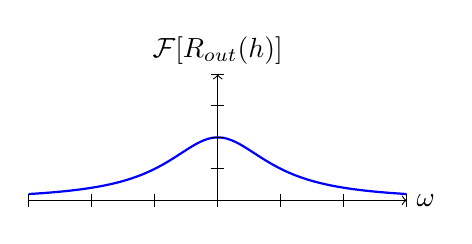
\begin{tikzpicture}[scale=0.8]
        % Draw axes
        \draw[->] (-3,0) -- (3,0) node[right] {$\omega$};
        \draw[->] (0,0) -- (0,2) node[above] {$\mathcal{F}[R_{out}(h)]$};
        % Plot Lorentzian: for illustration, set \kappa^2=1 and \gamma=1 so that f(\omega)=1/(1+\omega^2)
        \draw[blue, thick, domain=-3:3, samples=100] plot (\x,{1/(1+\x*\x)});
        % Add tick marks on the x-axis
        \foreach \x in {-3,-2,-1,0,1,2,3}
            \draw (\x,0.1) -- (\x,-0.1);
        % Add tick marks on the y-axis
        \foreach \y in {0,0.5,1,1.5,2}
            \draw (0.1,\y) -- (-0.1,\y);
    \end{tikzpicture}
    Right: $\mathcal{F}[R_{out}(h)] = \dfrac{\kappa^2}{\gamma^2+\omega^2}$.
    \end{minipage}
\end{figure}
    
    

